\documentclass[Bachelorarbeit.tex]{subfiles}
\begin{document}
\chapter{Literature Analysis}
The literature analysis began with the topic selection (see chapter \ref{ProblemDescription}). The supervisor told us that the initial chosen topic \textit{Face Detection} is to big to treat within one semester, so the first literature research was done to find a specific topic to handle.\\
The second literature research was done to find information about the chosen topic.
\section{Approach}
All interesting literature which were found and marked as interesting (by scanning the abstract) were saved in a list on the \href{https://ilias.fhv.at/goto.php?target=wiki_298249_Literature_Research_%28LR%29}{Ilias project space}. This articles were read in a more detail afterwards.\\
The structure of the table (see figure \ref{LRT}  make additional sorting (by exporting/copying into an EXCEL) possible and the implementation on ILIAS makes it possible to get access easily to the actual table.

\begin{figure}[!h] %LR table
\centering
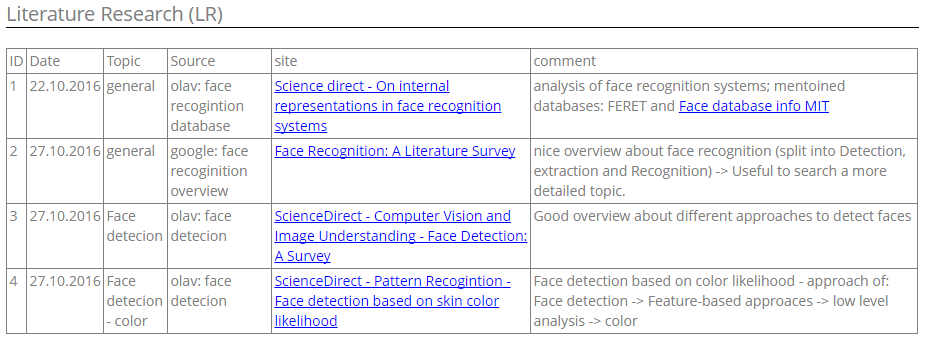
\includegraphics[width=10cm]{./pictures/LR_20161030}
\caption{Literature reasarech table - 30.10.2016. \label{LRT}}
\end{figure}

All literatures which were mentioned in this document are also listed in the bibliography.

\section{Literature analysis of the topic face detection based on color likelihood}
documentation why articles have been selected or rejected. All
used sources must be mentioned here
\end{document}